\documentclass[4paper]{article}
\usepackage[spanish]{babel}
%\usepackage[ansinew]{inputenc}
\usepackage[utf8x]{inputenc}
%\usepackage[utf-8]{inputenc}
%\usepackage[T1]{fontenc}
\usepackage{graphicx}
\usepackage{multicol}
%\usepackage{longtable}
%\usepackage{array}
%\usepackage{multirow}
%\usepackage[latin1]{inputenc}
%\inputencoding{latin1}

\renewcommand{\tablename}{Tabla}
\author{Manuel Molino Milla \and Luis Molina Garzón}
\title{\textbf{Programación}
\\COLECCIONES BÁSICAS}
\date{\today}

\begin{document}
\maketitle
%\tableofcontents
%\setlongtable 


\section*{Ejercicio 1}
¿Cuales de las siguientes sentencias son validas para la declaración de un array:
\begin{itemize}
\item int i = new int(30);
\item double d[ ] = new double[30];
\item char[ ] r = new char(1..30);
\item int i[ ] = (3, 4, 3, 2);
\item float f[ ] = \{2.3, 4.5, 6.6\};
\item char[ ] c = new char();
\end{itemize}

\section*{Ejercicio 2}
Crea una clase denominada Colecciones1, que tenga como atributo un array y que el constructor inicialize dicho array para almacenar doce valores de tipo double. Posteriormente en una clase denominada \emph{testColecciones1}:
\begin{itemize}
\item Asigna el valor 5 al último elemento.
\item Asigna el resto de valores con un bucle que el primer elemento sea 3 y los restantes el doble del anterior (el último elemento debe mantener el valor 5).
\item Mediante un bucle calcula la suma de todos los elementos del array.
\item Cambia el valor del array y divide por 3 todos los último cinco valores.
\item Calcula ahora el valor mas pequeño almacenado en el array.
\item Muestra todos los valores en tres filas de cuatro columnas, con una separación de cinco espacios.
\end{itemize}

\section*{Ejercicio 3}
Queremos leer los datos de temperaturas durante una semana y queremos almacenar dichos datos en un \emph{array}, para esto realiza una clase denominada \emph{Datos} teniendo en cuenta:
\begin{itemize}
\item Dicho \emph{array} como atributo de la clase.
\item Un constructor que inicialize dicho \emph{array}. Como argumento debemos pasar un array con siete valores.
\item Varios métodos que nos den los siguientes valores estadisticos:
\begin{itemize}
\item El \emph{valor medio} de dichos datos.
\item La \emph{desviación tipica}.
\item Numero de datos que se encuentran por debajo de la media.
\item El valor minimo.
\item El valor maximo.
\end{itemize}
\item Crea una nueva clase denominada \emph{TestDatos}, que lea los datos como parámetros (inventate dichos datos) y los añada a una \emph{ArrayList} de \emph{Double}, posteriormente convierte dicha \emph{ArrayList} a \emph{array} (mira en Internet como se puede hacer) y pásalo al constructor de la clase \emph{Datos}.
\item Crea un diagrama UML de la clase \emph{Datos}.
\item Documenta la clase \emph{Datos} mediante \emph{javadoc}
\end{itemize}


\section*{Ejercicio 4}
Queremos realizar un inventario de productos de oficina. Para esto crea las siguientes clases que indica el digagrama UML. En la clase \emph{Tienda}, el constructor inicializa la lista a vacía. Y en el caso de \emph{TestTienda} lee los productos usando la clase \emph{Scanner}.
\begin{figure}
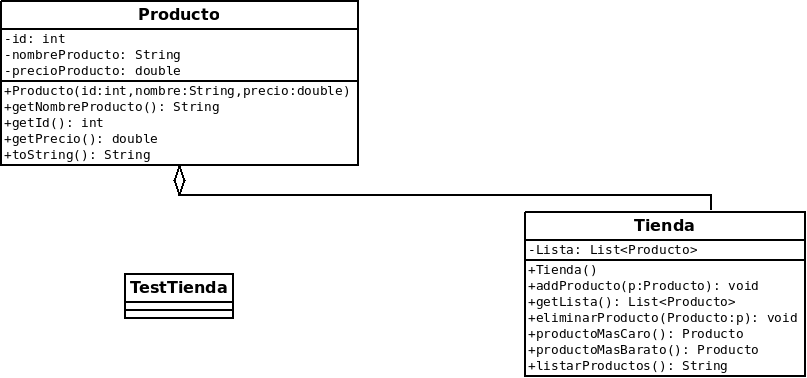
\includegraphics[scale=0.53]{ejercicio.png}
\caption{Diagrama UML del ejercicio}
\end{figure}

\end{document}
